\chapter{O poder dos números}
\label{les:15}

\begin{chapquote}{Lewis Carroll, \textit{Alice no País das Maravilhas}}
\enquote{Deixe-me ver: quatro vezes cinco é doze, e quatro vezes seis é treze, e quatro vezes sete é… ai, ai! deste jeito nunca vou chegar a vinte!}
\end{chapquote}

Os números são uma parte essencial do nosso dia a dia. Números grandes, entretanto, não são algo com que a maioria de nós esteja muito familiarizado. Os maiores números que podemos encontrar na vida cotidiana estão na faixa de milhões, bilhões ou trilhões. Podemos ler sobre milhões de pessoas na pobreza, bilhões de dólares gastos em resgates aos bancos e trilhões de dívidas nacionais. Embora seja difícil entender essas manchetes, estamos um tanto quanto confortáveis com o tamanho desses números.

Embora possamos parecer confortáveis com bilhões e trilhões, nossa intuição já começa a falhar com números dessa magnitude. Você tem uma intuição de quanto tempo teria que esperar para que um milhão/bilhão/trilhão de segundos passassem? Se você for como eu, você está perdido sem realmente analisar os números.

Vamos dar uma olhada neste exemplo: a diferença entre cada um é um aumento de três ordens de magnitude: $10^6$, $10^9$, $10^{12}$. Pensar em segundos não é muito útil, então vamos traduzir isso em algo que possamos entender com mais clareza:

\begin{itemize}
  \item $10^6$: Um milhão de segundos são $5$ semanas e meia.
  \item $10^9$: Um bilhão de segundos são aproximadamente 32 anos.
  \item $10^{12}$: Um trilhão de segundos no passado, Manhattan estava coberta por uma camada grossa de gelo.\footnote{Um trilhão de segundos ($10^{12}$) atrás, estávamos a $31710$ anos no passado. A última Era Glacial foi a $33,000$ anos.~\cite{wiki:LGM}}
\end{itemize}

\begin{figure}
  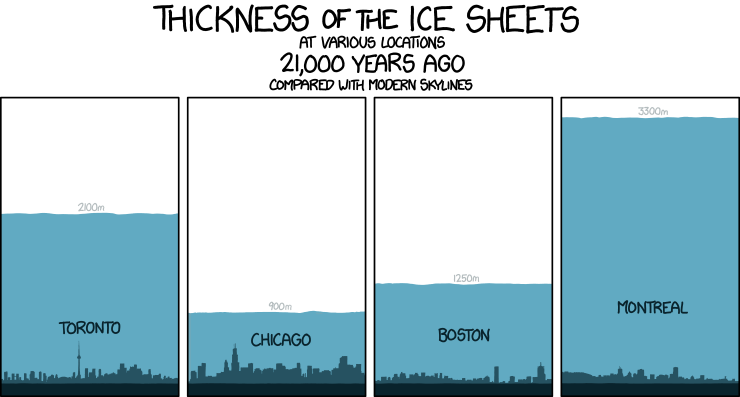
\includegraphics{assets/images/xkcd-1225.png}
  \caption{Um trilhão de segundos no passado. Fonte: xkcd 1225}
  \label{fig:xkcd-1225}
\end{figure}

Assim que entramos na escala astronômica da criptografia moderna, nossa intuição falha catastroficamente. O Bitcoin é construído em torno de grandes números e da impossibilidade virtual de adivinhá-los. Esses números são muito, muito maiores do que qualquer coisa que possamos encontrar no nosso dia a dia. Muitas ordens de magnitude maiores. Entender o quão grandes esses números realmente são é essencial para entender o Bitcoin como um todo.

Vamos pegar o SHA-256\footnote{O SHA-256 faz parte da família SHA-2 de funções criptográficas de hash desenvolvidas pela NSA.~\cite{wiki:sha2}}, uma das funções hash\footnote{O Bitcoin usa SHA-256 em seu algoritmo de hashing de bloco.~\cite{btcwiki:block-hashing}} usado no Bitcoin, como um exemplo concreto. É natural pensar em 256 bits como \enquote{duzentos e cinquenta e seis}, que não é um número grande. No entanto, o número depois do SHA-256 está falando sobre ordens de grandeza --- algo com que nossos cérebros não estão bem equipados para lidar.

Embora o comprimento do bit seja uma métrica conveniente, o verdadeiro significado da segurança dos 256 bits se perde na tradução. Semelhante aos milhões ($10^6$) e bilhões ($10^9$) acima, o número do SHA-256 é de ordem de grandeza ($2^{256}$).

Então, qual é a força do SHA-256, exatamente?

\begin{quotation}\begin{samepage}
\enquote{SHA-256 é muito forte. Não é como uma etapa incremental que podemos ver do MD5 para o SHA1. Pode durar várias décadas, a menos que haja algum avanço no ataque.}
\begin{flushright} -- Satoshi Nakamoto\footnote{Satoshi Nakamoto, em resposta a pergunta sobre as colisões no SHA-256. \cite{satoshi-sha256}}
\end{flushright}\end{samepage}\end{quotation}

Vamos esclarecer as coisas. $2^{256}$ é igual ao seguinte número:

\begin{quotation}\begin{samepage}
    115 quatuorvigintilhão 792 trevigintilhões 89 duovigintilhões 237 unvigintilhões 316 vigintilhões 195 novemdecilhões 423 octodecilhões 570 septendecilhões 985 sexdecilhões 8 quindecilhões 687 quatuordecilhões 907 tredecilhões 853 duodecilhões 269 undecilhões 984 decilhões 665 nonilhões 640 octilhões 564 septilhões 39 sextilhões 457 quintilhões de 584 quatrilhões 7 trilhões 913 bilhões 129 milhões 639 mil 936.
\end{samepage}\end{quotation}

São muitos nonilhões! Tentar fazer com que esse número entre na sua cabeça é praticamente impossível. Não há nada no universo físico para compararmos. É muito maior do que o número de átomos no universo observável. O cérebro humano simplesmente não foi feito para dar sentido a essa magnitude.

\newpage

Uma das melhores visualizações da verdadeira força do SHA-256 é um vídeo de Grant Sanderson. Apropriadamente nomeado \textit{\enquote{Quão forte é a segurança de 256 bits?}}\footnote{Assista ao vídeo acessando o link \url{https://youtu.be/S9JGmA5_unY}}, onde ele mostra maravilhosamente o quão grande é um número de 256 bits. Faça um favor a si mesmo e reserve cinco minutos para assisti-lo. Como todos os outros vídeos do \textit{3Blue1Brown}, este não é apenas fascinante, mas também excepcionalmente bem feito. Aviso: você pode cair na toca do coelho da matemática.

\begin{figure}
  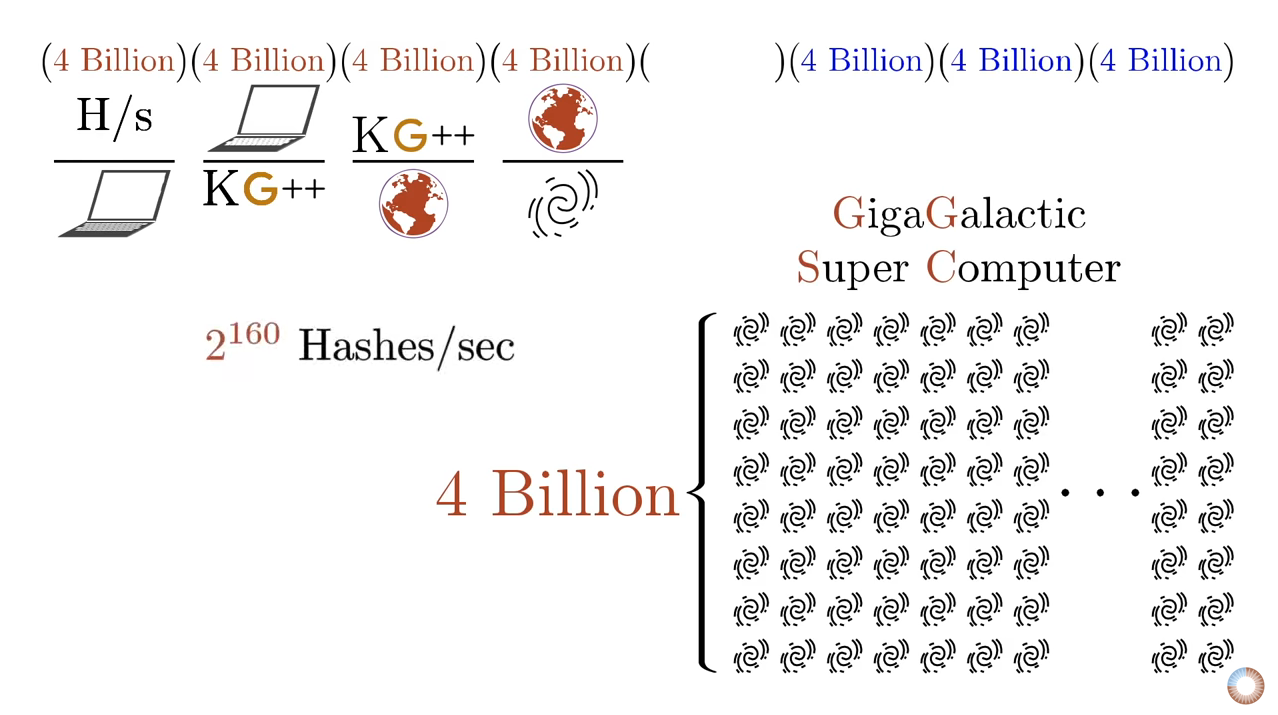
\includegraphics{assets/images/youtube-vid-inverted.png}
  \caption{Ilustração da segurança do SHA-256. Gráfico original feito por Grant Sanderson, conhecido como 3Blue1Brown.}
  \label{fig:youtube-vid-inverted}
\end{figure}

Bruce Schneier~\cite{web:schneier} usou os limites físicos da computação para colocar este número em perspectiva: mesmo que consigamos construir um computador perfeito, que poderia usar energia proveniente de qualquer tipo de matriz energética para mudar perfeitamente os bits~\cite{wiki:landauer}, mesmo que possamos construir uma esfera de Dyson\footnote{Uma esfera Dyson é uma mega estrutura hipotética que poderia envolver uma estrela e capturar uma grande porcentagem da sua energia emanada.~\cite{wiki:dyson}} envolta do sol, e deixar este computador rodando por 100 bilhões de bilhões de anos, ainda teríamos apenas $25\%$ de chance de encontrar a agulha no palheiro de 256 bits.

\begin{quotation}\begin{samepage}
\enquote{Estes números não tem nada ver com a tecnologia dos nossos dispositivos; eles são o máximo que a termodinâmica nos permite. E eles implicam fortemente que, um ataque de força bruta contra chaves de 256 bits seja inviável até que os computadores possam ser construídos com alguma coisa além da matéria e, que ocupem algo mais do que o espaço físico que conhecemos.}
\begin{flushright} -- Bruce Schneier\footnote{Bruce Schneier, \textit{Applied Cryptography} \cite{bruce-schneier}}
\end{flushright}\end{samepage}\end{quotation}

É difícil exagerar a profundidade disso. A forte criptografia inverte o equilíbrio de poder do mundo físico com o qual estamos tão acostumados. Coisas inquebráveis não existem no mundo real. Aplique uma força suficiente e poderemos abrir qualquer porta, caixa ou baú de tesouro.

O baú do tesouro do Bitcoin é muito diferente. É protegido por uma criptografia fortíssima, que não dá lugar à força bruta. E, enquanto as suposições matemáticas se mantiverem, a força bruta é tudo o que temos. Existem também a opção de um ataque global, usando uma chave inglesa de \$5 dólares (Figura~\ref{fig:xkcd-538}), mas a tortura não funcionará para todos os endereços do Bitcoin, e as paredes criptográficas dessa moeda derrotarão os ataques de força bruta. Mesmo se alguém tente atacar com a força de mil sóis. Literalmente.

\begin{figure}
  \centering
  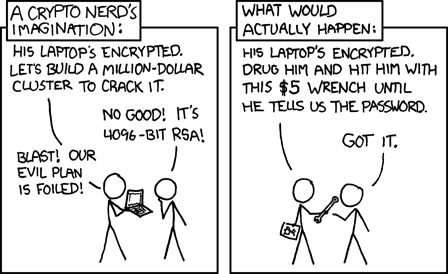
\includegraphics[width=8cm]{assets/images/xkcd-538.png}
  \caption{Ataque de chave inglesa de \$5 dólares. Fonte: xkcd 538}
  \label{fig:xkcd-538}
\end{figure}

Este fato e suas implicações foram resumidos de forma pujante no chamado a guerra criptográfica: \textit{\enquote{Nenhuma quantidade de força coercitiva resolverá um problema matemático.}}

\begin{quotation}\begin{samepage}
\enquote{Não é óbvio que o mundo teve que funcionar dessa maneira. Mas de alguma forma o universo sorri com a criptografia.}
\begin{flushright} -- Julian Assange\footnote{Julian Assange, \textit{A Call to Cryptographic Arms} \cite{call-to-cryptographic-arms}}
\end{flushright}\end{samepage}\end{quotation}

Ninguém ainda sabe ao certo se o sorriso do universo é genuíno ou não. É possível que nossa suposição de assimetrias matemáticas esteja errada e então descobriremos que P na verdade é igual a NP \cite{wiki:pnp}, ou encontraremos soluções surpreendentemente rápidas para problemas específicos \cite{wiki:discrete-log} que atualmente assumimos serem difíceis. Se for esse o caso, a criptografia como a conhecemos deixará de existir e as implicações provavelmente mudariam o mundo como o conhecemos hoje.

\begin{quotation}\begin{samepage}
\enquote{Vires in Numeris} = \enquote{Força nos Números}\footnote{\textit{Vires in Numeris} foi a primeira proposta de lema para o Bitcoin, feita pelo usuário \textit{epii}~\cite{epii} no fórum bitcointalk.}
\end{samepage}\end{quotation}

\textit{Vires in numeris} não é apenas um lema cativante usado pelos bitcoinheiros. A compreensão de que existe uma força que não pode ser freada e que foi encontrada nos números é profunda. Entender isso e a inversão dos equilíbrios de poder existentes foi o que permitiu mudar minha visão de mundo e do futuro que está à nossa frente.

Um resultado direto disso é o fato de que você não precisa pedir permissão a ninguém para participar do Bitcoin. Não existe uma página para se inscrever, nenhuma empresa responsável, nenhuma agência governamental para enviar os formulários de inscrição. Basta gerar um grande número e você estará pronto para prosseguir. A autoridade central de criação de contas é a matemática. E só Deus sabe quem está encarregado disso.

\begin{figure}
  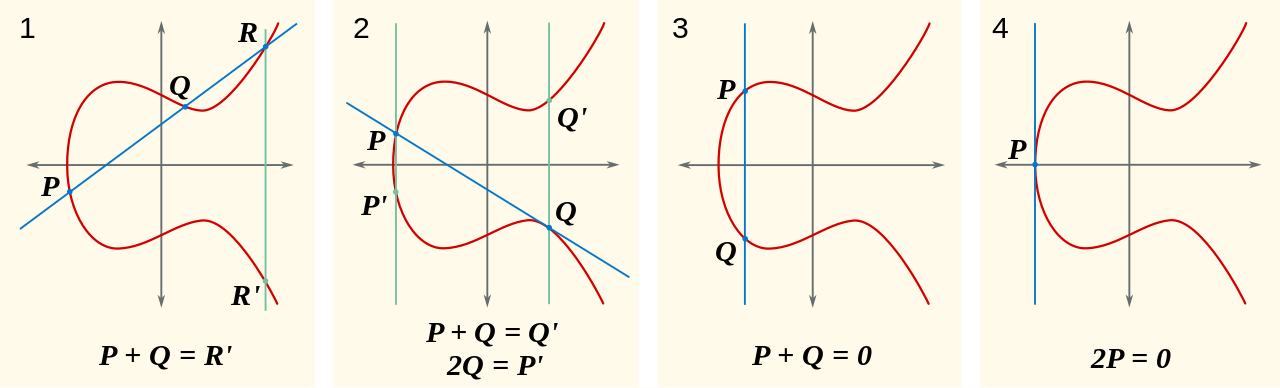
\includegraphics{assets/images/elliptic-curve-examples.png}
  \caption{Exemplo de curvas elípticas. Gráficos sob a licença de cc-by-sa disponibilizadas por Emmanuel Boutet.}
  \label{fig:elliptic-curve-examples}
\end{figure}

O Bitcoin é construído com base em nosso melhor entendimento da realidade. Embora ainda existam muitos problemas abertos na física, ciência da computação e matemática, temos muita certeza sobre algumas coisas. Existe uma assimetria entre encontrar soluções e validar a correção dessas soluções. Isso é uma dessas coisas. Essa computação precisar de energia, é outra. Em outras palavras: encontrar uma agulha em um palheiro é mais difícil do que verificar se a coisa pontuda em sua mão é mesmo uma agulha ou não. E encontrar a agulha dá um trabalhão.

A vastidão do espaço de endereços do Bitcoin é verdadeiramente estonteante. O número de chaves privadas é ainda mais. É fascinante como muito de nosso mundo moderno se resume à improbabilidade de encontrar uma agulha em um palheiro incomensuravelmente grande. Agora estou mais ciente desse fato do que nunca.

\paragraph{O Bitcoin me ensinou que existe força nos números.}

% ---
%
% #### Down the Rabbit Hole
%
% - [How secure is 256 bit security?]["How secure is 256 bit security?"] by 3Blue1Brown
% - [Block Hashing Algorithm][hash functions] on the Bitcoin Wiki
% - [Last Glacial Maximum][thick layer of ice], [SHA-2][SHA-256], [Dyson Sphere][Dyson sphere], [Landauer's Principle][flip bits perfectly] [P versus NP][P actually equals NP], [Discrete Logarithm][specific problems] on Wikipedia
%
% [thick layer of ice]: https://en.wikipedia.org/wiki/Last_Glacial_Maximum
% [xkcd \#1125]: https://xkcd.com/1225/
% [SHA-256]: https://en.wikipedia.org/wiki/SHA-2
% [hash functions]: https://en.bitcoin.it/wiki/Block_hashing_algorithm
% ["How secure is 256 bit security?"]: https://www.youtube.com/watch?v=S9JGmA5_unY
% [Bruce Schneier]: https://www.schneier.com/
% [flip bits perfectly]: https://en.wikipedia.org/wiki/Landauer%27s_principle#Equation
% [Dyson sphere]: https://en.wikipedia.org/wiki/Dyson_sphere
% [2]: https://books.google.com/books?id=Ok0nDwAAQBAJ&pg=PT316&dq=%22These+numbers+have+nothing+to+do+with+the+technology+of+the+devices;%22&hl=en&sa=X&ved=0ahUKEwjXttWl8YLhAhUphOAKHZZOCcsQ6AEIKjAA#v=onepage&q&f=false
% [wrench attack]: https://xkcd.com/538/
% [call to cryptographic arms]: https://cryptome.org/2012/12/assange-crypto-arms.htm
% [P actually equals NP]: https://en.wikipedia.org/wiki/P_versus_NP_problem#P_=_NP
% [specific problems]: https://en.wikipedia.org/wiki/Discrete_logarithm#Cryptography
% [3Blue1Brown]: https://twitter.com/3blue1brown
%
% <!-- Wikipedia -->
% [alice]: https://en.wikipedia.org/wiki/Alice%27s_Adventures_in_Wonderland
% [carroll]: https://en.wikipedia.org/wiki/Lewis_Carroll
